\chapter{Introduction}
\label{chapter:introduction}
The history of a particle physics is a fascinating jurney towards the smallest, the most principle elements of the Universe. Starting from memorable Rutheford experiment in 1909 \cite{Rutheford} up to Higss boson discovery \cite{Higgs_CMS, Higgs_ATLAS}, and misterous states X,Y,Z [ref] oserved at the begining of XXIth century. Throughout this entire jurney there were many attemps to point out which particles are realy elementery, and classify them. Nowadays the knowledge about elementary particles is collected in theory colled the standart model (SM) which describes almost all known particles and interaction between them.

According to the Standard Model we can divide elementary particles into three groups: leptons and quarks, basic bricks of the universe and elementary bosons a force-carryng particles. In contrary to leptons bosons can not exist in the nature in free states. This phenomena called ``a confiment'' is still not fully understood. Nonetheless, as a result ot the confiment, we can observe quarks in bound states: mesons and baryions. Mesons have a baryonic number equal 0 and mostly consist of two quarks. However such an exotic object like glueball are also classyfied as mesons. Baryons are characterized by barionic number different than 0. Commonly obsered in nature consist of three quarks, but rare objects, like pentaquark, also belong to baryions.

A quark model proposed by Gell-Mann and Zweig in 1964 \cite{Gell-Mann,Zweig} describes well a hierarchy of ground barionic nad masonic states. However to discribe origin of paricles properties like mass or spin, and predict excited states, a theory of quarks dynamics is required. Interaction between quarks are dominated by the strong force. Its general descripction, given by quantum chromo-dynamisc is very demanding in scpecific problems. For high energy regime an asymptotic freedom allows to solve equation by a series expansion. For low energys two approaches are possible: a phenomenological models, or a lattice calculations. Especially a barionic spectrum is poorly known and requires further investigations.



\section{Hyperons}
Assuming that energy avaliable in the system is below a  $\mathrm{J/\psi}$ messon mass (3.1 GeV/c) we can acknowledge that all the matter is built of three types of quarks: up, down and strange. These quarks are treated in quark model as an irreduciable representation of a SU3 symmetry group. The possible ground states for a three-quarks systems have been predicted by quark model and described by the baryon octet and the baryon decuplet. All baryons consisting a strange quark are called hyperons.  

\begin{figure}[hb]
  \centering
  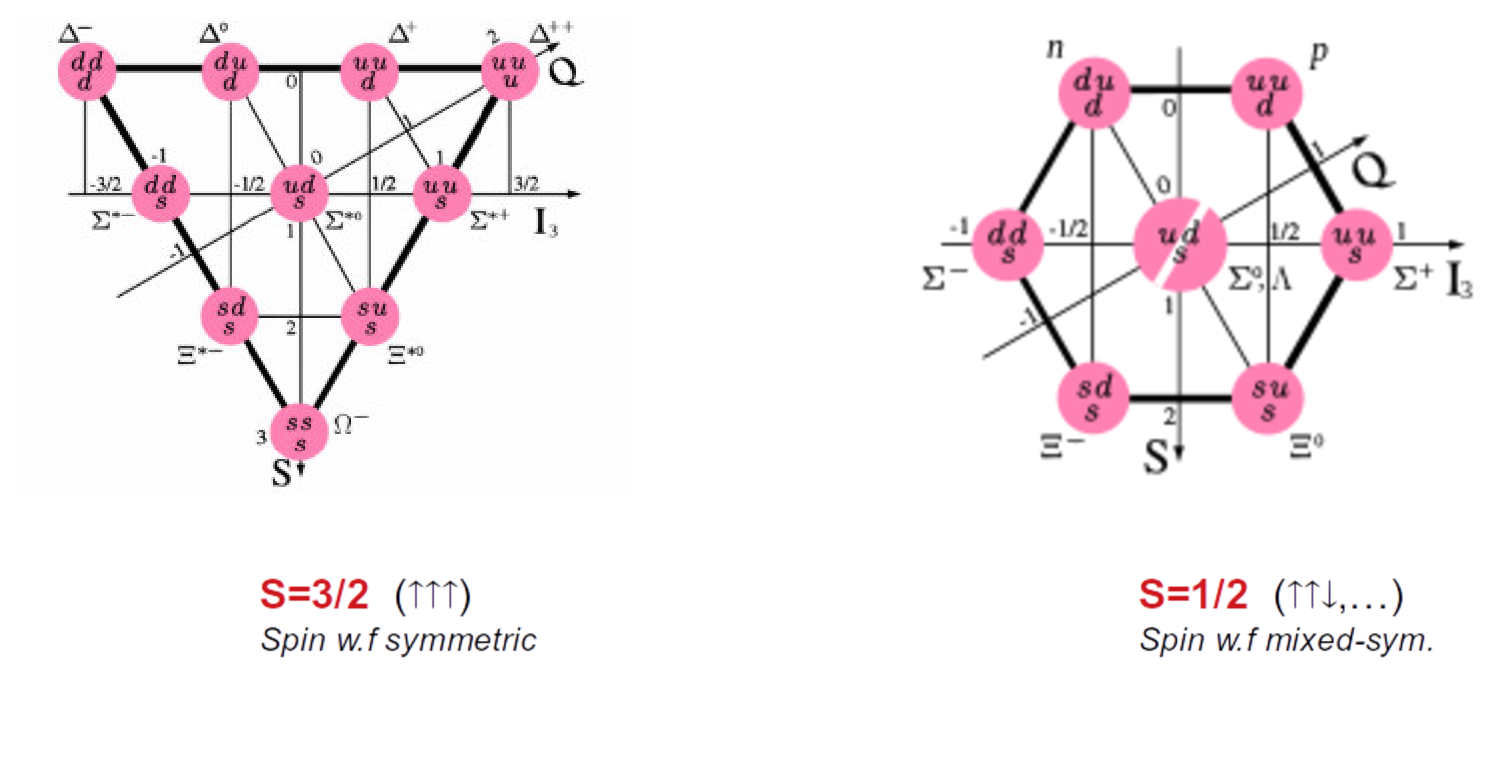
\includegraphics[width=0.9 \linewidth]{Chapter_introduction/eightfolds.eps}
  \caption{The eightfolds proposed by Gell-Mann and Ne'eman in 1961 to clasyfy baryonic states. At a publication moment they classyfy all known baryions except the $\Omega^-$. Its discovery in 1964 \cite{omega} was a great success of the quark model. }
  \label{fig:eigh}
\end{figure}

The quark modell is very succesful in a description of the baryonic ground states. However it gives no clue about excited states and quarks dynamics inside a particle. Because lattice QCD is still not able to reproduce even ground states masses the hyperons spectrum is calculated using effective theoris [ref]. Despite a huge theoretical end experimental effort a theoretical predictions and experimental data are still far away from agreement, especially in high mass range. The example of such is presented in fig. \ref{fig:spectrum}.

\begin{figure}[hb]
  \centering
  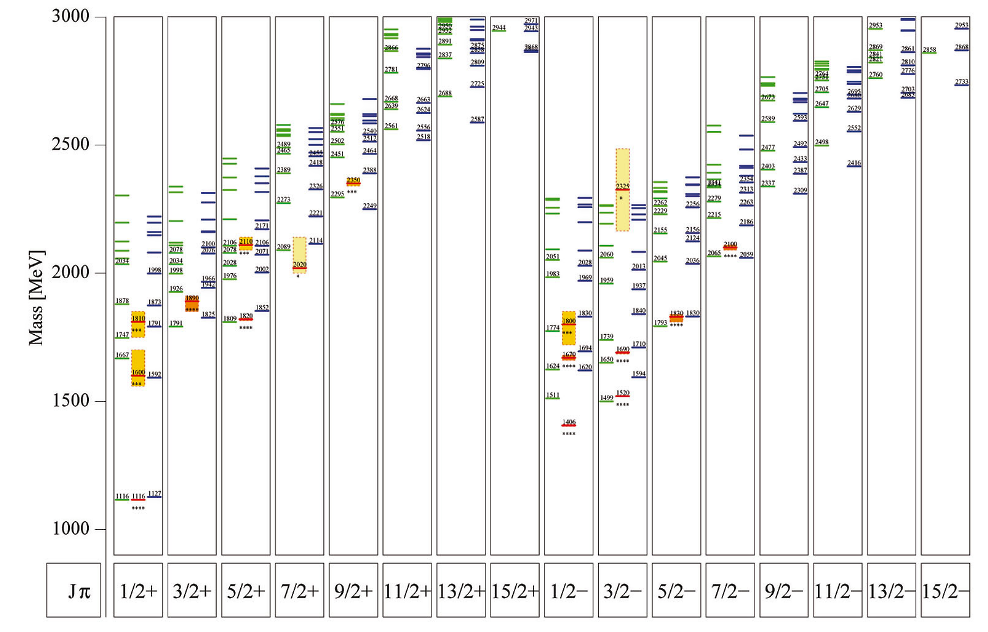
\includegraphics[width=0.99 \linewidth]{Chapter_introduction/spectrum.png}
  \caption{The comparison of experimental data (middle column) and theoretical predictions (left, and right column) of relativistically covariant constituent quark models for $\Lambda$ hyperons. The picture shows how limited is our experimental knowledge compare to theroetical predictions. The picture is taken from \cite{Ronniger2012}}
  \label{fig:spectrum}
\end{figure}
\section{Form factors}
Any kind of a scattering experiment performed to examinate physics inside baryions faces a fundamental problem of a rich internal structure of them. An complicated interactions inside the baryon can be treatet together and their inpact on a scattering could be take into consideration by one scalar function called a form factor F(q),
\begin{equation}
  \frac{d \sigma}{d \Omega}=\left( \frac{d \sigma}{d \Omega}\right)_{point-like} |F(\vec{q})|^2.
\end{equation}
As long as a target is static and spin-less the form factor is a the Fourier Transform of the charge decsity in target,
\begin{equation}
  F(\vec{q})=\int \rho(\vec{x}) e^{i \vec{q} \cdot \vec{x}}d^3x.
\end{equation}
Practically this relation occures whent a target is much heavier than a projectle, like in Rutheford experiment \cite{Rutheford}. In case of electron on proton scattering situation is more complicated because both particles has a spin and a proton gets recoil after scattering. A solution for this problem is called the Rosenbluth formula and looks as follows
\begin{equation}
  \frac{d \sigma}{d \Omega}\bigg|_{lab}=\left(\frac{\alpha^2}{4E^2 \mathrm{sin}^4 \frac{\theta}{2}}\right) \frac{E'}{E} \left[ \left(F_1(q^2)^2- \frac{\kappa^2 q^2}{4M^2} F_2(q^2)^2\right) \mathrm{cos}^2\frac{\theta}{2}-\frac{q^2}{2M^2} \left(F_1(q^2) + \kappa F_2(q^2)\right)^2 \mathrm{sin}^2 \frac{\theta}{2} \right],
\end{equation}
where $F_1(q^2)$ and $F_2(q^2)$ are two independent form factors, $\kappa$ anomalus magnetic moment, $q$ a four-momentum transfer. Factor
\begin{equation}
  \frac{E'}{E}=\frac{1}{1+\frac{2E}{M}\mathrm{sin}^2\frac{\theta}{2}}
\end{equation}
is conected with the proton recoil. Because functions $F_1$ and $F_2$ form an interference term it is convinient to express them as a linear combination of $G_e$ and $G_M$.
\begin{equation}
  G_e=F_1+\frac{\kappa q^2}{4M^2}F_2
\end{equation}
\begin{equation}
  G_M=F_1+\kappa F_2
\end{equation}

\section{Dalitz decays}
The idea of form-fastrs was introduced first time in context of scattering experiments. A Faynmann diagram for such phenomena is shown in fig. \ref{fig:FF_kinds} a). Due to kinematic constrains for the scattering a four-momentum $q^2$ is always negative - a projectile transfers part of its four-momentum into target. However an idea of the form factor can be extendet to annichilation experiments, where $q^2>0$ (fig.\ref{fig:FF_kinds} b)). Unfortunatelly, to produce a baryion-antybaryion pair energy equal at least their mases is reqired. It measns that $q^2$ can not be smaller than $4M_b^2$. This gap in $q^2$ can be explored in a range $0<q^2<4M_b^2$ by process called a Dalitz decay. 

\begin{figure}[hb]
  \centering
  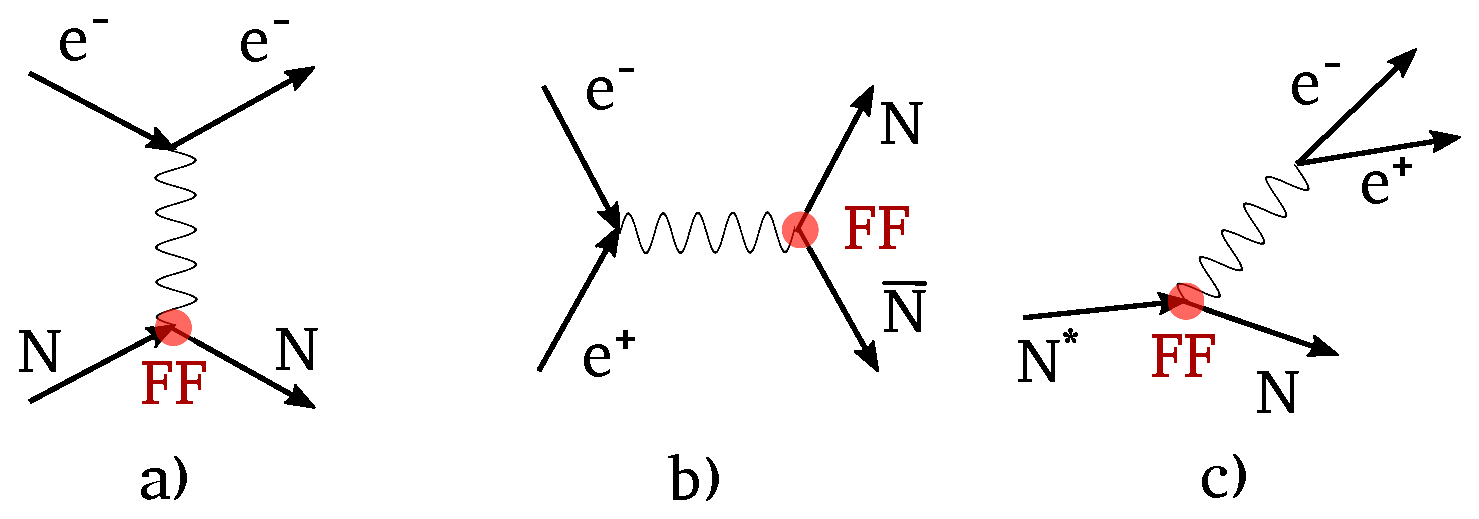
\includegraphics[width=0.9 \linewidth]{Chapter_introduction/faynmannDiagrams.eps}
  \caption{Three processes involving a nucleon electromagnetic form factors: a) an electron-nucleon scattering, b) an electron-positron anichilation, c) a nucleon Dalitz decay.}
  \label{fig:FF_kinds}
\end{figure}

The Dalitz decay of a nucleon ( is fig.\ref{fig:FF_kinds} c)) is a reaction 